\documentclass[a4paper,titlepage]{article}

\usepackage[final]{changes}

\usepackage{hyperref}
\usepackage{amsmath}
\usepackage{amssymb}
\usepackage{braket}
\usepackage{siunitx}
\DeclareSIUnit\angstrom{\text{\AA}}
\usepackage[version=4]{mhchem}
\usepackage{tikz}
\usetikzlibrary{positioning}
\usetikzlibrary {arrows.meta} 
\usepackage{paralist}
\usepackage{todonotes}
\usepackage{tabularray}
\usepackage{booktabs}


\renewcommand{\thetable}{S\arabic{table}}
\renewcommand{\thefigure}{S\arabic{figure}}
\renewcommand\thepage{S\arabic{page}}


\title{Theoretical study of reduction reactions near a calcium anode: a grand canonical DFT investigation\\Supporting information}

\author{Pierre Beaujean, Benoît Champagne}

\begin{document}
\maketitle

\begin{figure}[!h]
	\centering
	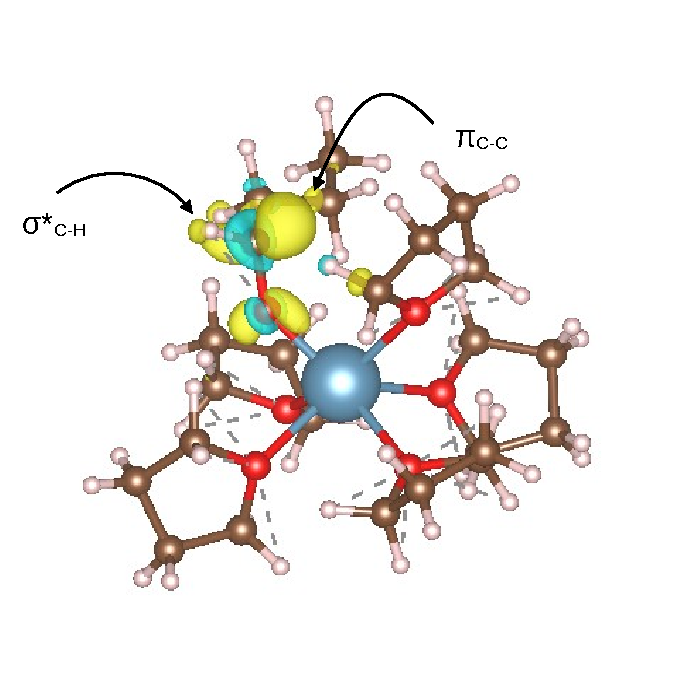
\includegraphics[width=\linewidth]{FigureS1}
	\caption{Spatial arrangement of the slab (Ca, top, \ce{CaH2}, bottom) + solvated \ce{Ca^2+} (\textbf{1\textsuperscript{2+}}) models. The unit cell is marked by  a dashed line.}
	\label{fig:spac}
\end{figure}

\begin{figure}[!h]
	\centering
	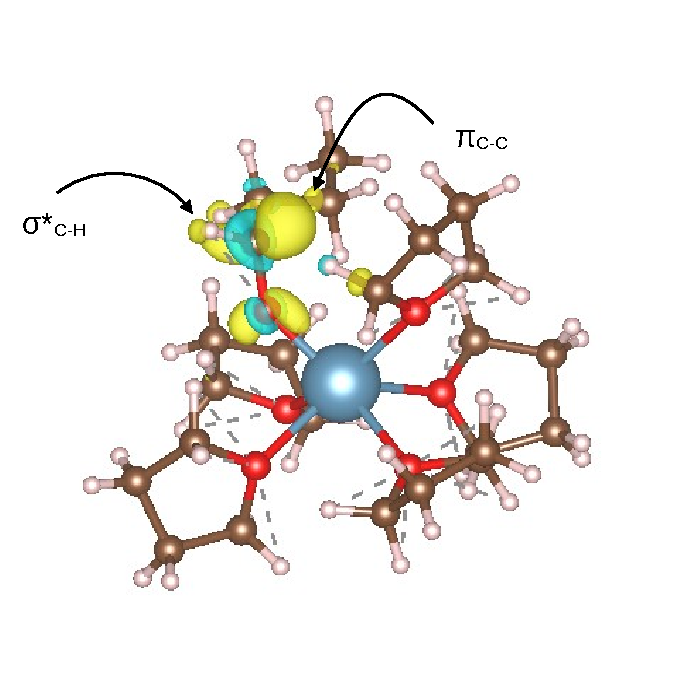
\includegraphics[width=\linewidth]{FigureS2}
	\caption{Electrostatic potential ($E_\infty$, top panel) and $xy$-averaged electron density ($\rho(r)$, bottom panel) along the surface normal for the simulation cell consisting of calcium slabs separated by \SI{52}{\angstrom}, with \textbf{1} positioned \SI{9}{\angstrom} above the surface and $\Delta n_e = \SI{0}{\elementarycharge}$. The vacuum region is highlighted.}
\end{figure}

\begin{figure}[!h]
	\centering
	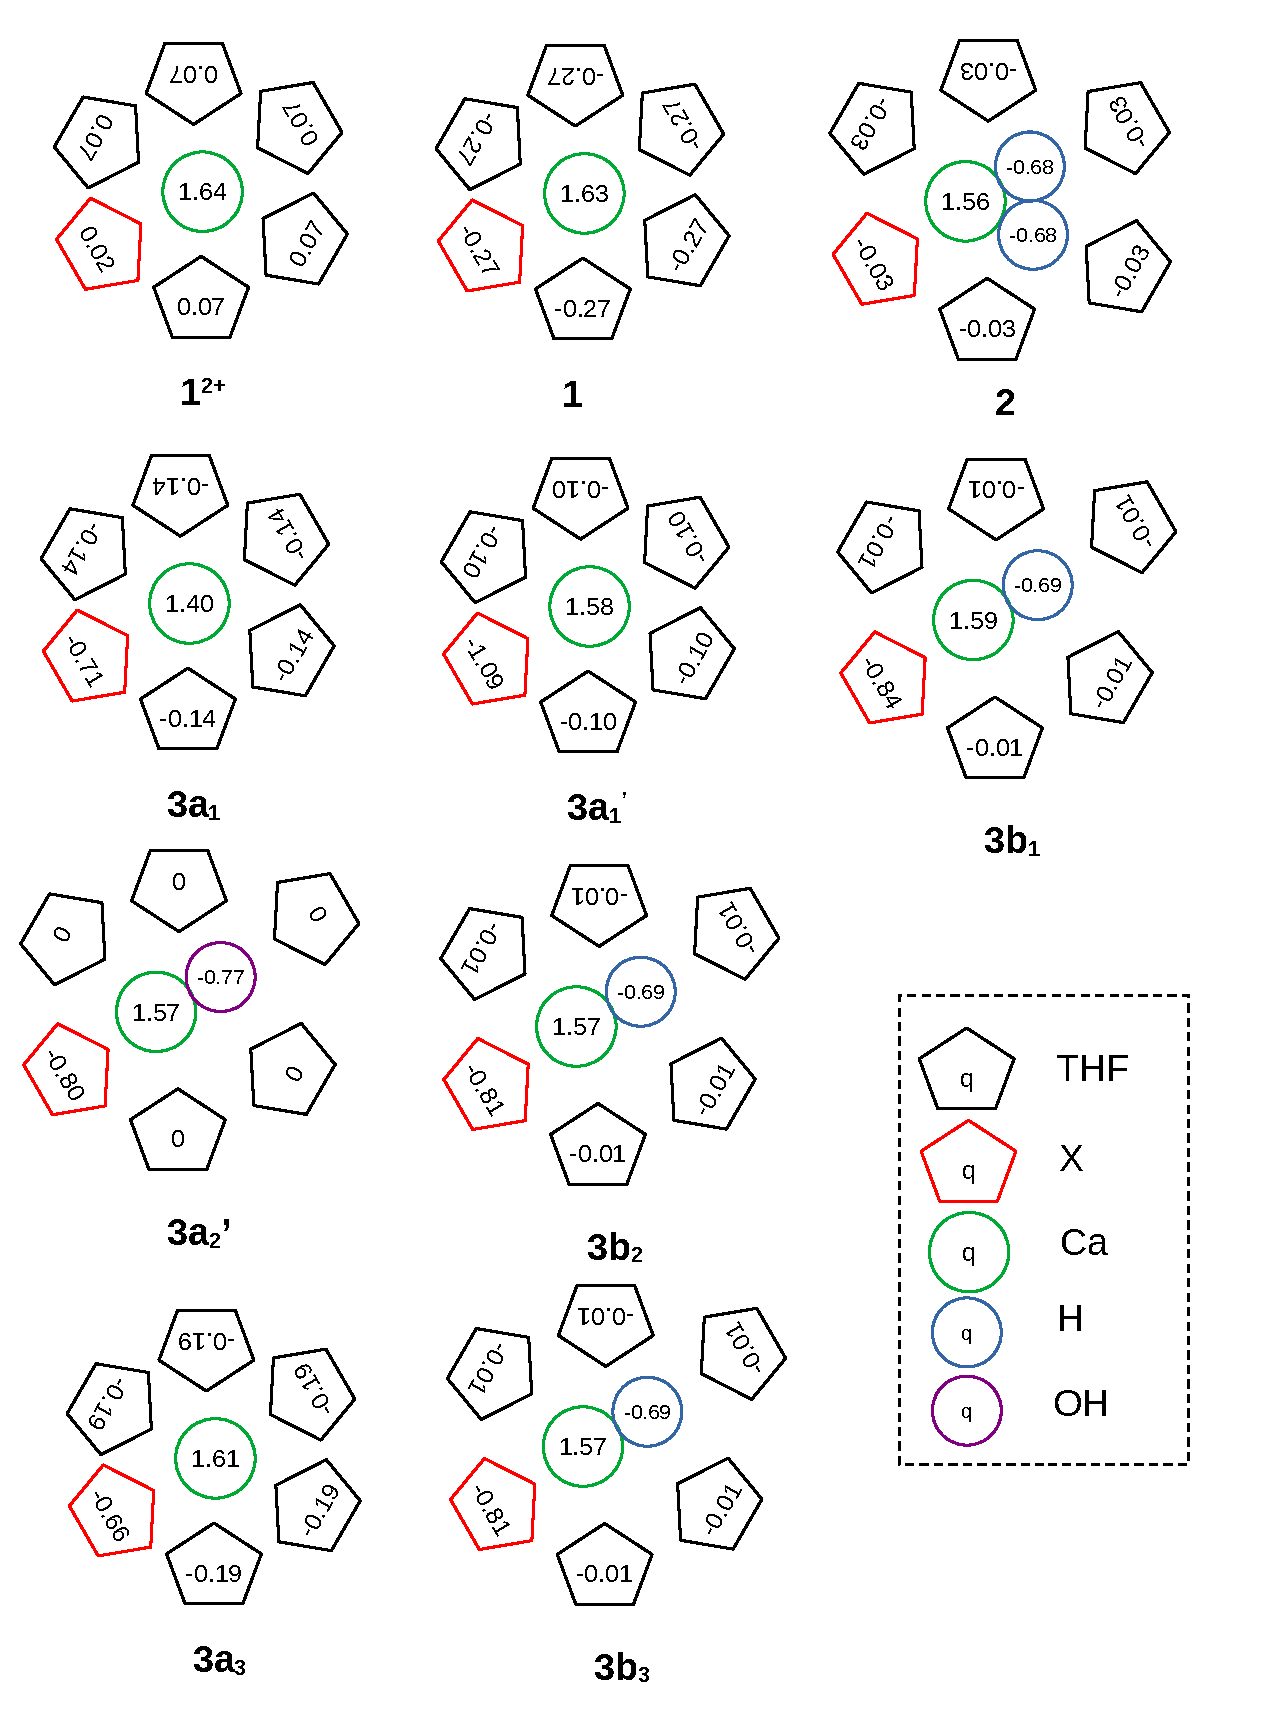
\includegraphics[width=\linewidth]{FigureS3}
	\caption{Effect of the interslab separation distance, $d$ (\si{\angstrom}), on the electrostatic potential ($E_\infty$, top panel) and the $xy$-averaged electron density ($\rho(r)$, middle panel) for a calcium slab with \textbf{1} positioned \SI{9}{\angstrom} above the surface (Fig.~\ref{fig:spac}) and $\Delta n_e = \SI{0}{\elementarycharge}$. The bottom panel shows the corresponding variation of the work function, $\Phi = E_\infty - E_F$, with $d$, where $E_F$ denotes the Fermi level.}
\end{figure}


\begin{table}
	\centering
	\begin{tabular}{>{\bfseries}l>{\bfseries}lcc}
		\toprule
		Line 1 & Line 2 & $E^0_{rel}$ & $F$ \\
		\midrule
		\multicolumn{4}{c}{Figure 1} \\
		\ce{Ca_{(surf)} + 6 THF} & \ce{Ca_{(surf)} + Ca(THF)6} & -3.439 & -1.855 \\
		\midrule
		\multicolumn{4}{c}{Figure 4} \\
		1 & bare & -3.396 & -1.872 \\
		1 & 3a\textsubscript{2}’ & -3.018 & -2.967 \\
		1 & 2 & -2.686 & -4.096 \\
		1 & 3b\textsubscript{1} & -1.424 & -9.372 \\
		1 & 3a\textsubscript{1}’ & -1.288 & -10.082 \\
		1 & 3b\textsubscript{2} & -1.232 & -10.360 \\
		1 & 3b\textsubscript{3} & -1.172 & -10.678 \\
		3a\textsubscript{1}’ & 3b\textsubscript{1} & -1.566 & -9.363 \\
		3a\textsubscript{1}’ & 3b\textsubscript{2} & -1.185 & -10.387 \\
		3a\textsubscript{1}’ & 3b\textsubscript{3} & -1.058 & -10.766 \\
		3b\textsubscript{3} & 3b\textsubscript{2} & -2.351 & -10.802 \\
		\midrule
		\multicolumn{4}{c}{Figure 6} \\
		1 & 3b\textsubscript{1}& -0.649 & -9.448 \\
		\bottomrule
		\end{tabular}
		\caption{List of all intersection between lines in electrochemical free energy ($F$, in \si{\electronvolt}) \textit{vs} electrode potential ($E^0_{rel}$, in \si{\volt}) graphs of the main text.}
\end{table}

\begin{table}
	\centering
	\begin{tabular}{>{\bfseries}lc c ccccc}
		\toprule
		& Ca--O[X] & & \multicolumn{5}{c}{Ca--O[THF]} \\
		\cmidrule{4-8}
		1 & 2.366 &  & 2.367 & 2.363 & 2.365 & 2.363 & 2.367 \\
		1\textsuperscript{2+} & 2.349 &  & 2.365 & 2.368 & 2.363 & 2.367 & 2.370 \\
		2 & 4.497 &  & 2.525 & 2.537 & 2.543 & 2.497 & 2.624 \\
		3a\textsubscript{1} & 2.394 &  & 2.511 & 2.574 & 2.539 & 2.549 & 2.505 \\
		3a\textsubscript{1}’ & 2.089 &  & 2.490 & 2.458 & 2.549 & 2.448 & 2.493 \\
		3b\textsubscript{1} & 2.185 &  & 2.584 & 2.688 & 2.597 & 2.534 & 2.580 \\
		3a\textsubscript{2}’ & 2.165 &  & 2.484 & 2.644 & 2.474 & 3.382 & 2.568 \\
		3b\textsubscript{2} & 2.162 &  & 2.522 & 2.691 & 2.578 & 2.528 & 2.768 \\
		3a\textsubscript{3} & 2.344 &  & 2.412 & 2.428 & 2.436 & 2.432 & 2.406 \\
		3b\textsubscript{3} & 2.108 &  & 2.528 & 2.676 & 2.487 & 2.589 & 2.984 \\
		\bottomrule
	\end{tabular}
	\caption{Calcium-oxygen distances (with the oxygen of each of the 5 \textit{intact} THF's, Ca--O[THF], and with the oxygen of the \textit{degraded} THF, Ca--O[X], in \si{\angstrom}) for all degradation reactions (\textbf{2}-\textbf{3}).}
	\label{tab:dists}
\end{table}

\begin{table}
	\centering
	\begin{tabular}{>{\bfseries}l ccc}
		\toprule
		&PBE-D3	&M06-2X&	$\omega$B97X-D\\
		\midrule
		3b\textsubscript{1}	&-5.36 (0.64)&	-5.46 (0.74)&	-5.29 (0.56) \\
		3b\textsubscript{2}	&-4.71 (0.67)&	-4.74 (0.70)&	-4.54 (0.50) \\
		3b\textsubscript{3}	&-4.63 (0.57)	&-4.69 (0.63)&	-4.48 (0.41) \\
		\bottomrule
	\end{tabular}
	\caption{Reduction reaction energies starting from \textbf{1\textsuperscript{2+}} ($\Delta E_r$, in \si{\electronvolt}) computed with the cc-pVTZ basis set and different exchange--correlation functionals using ORCA. Deviations from the corresponding PBE-D3/PAW values reported in Table 1 of the main text are given in parentheses. Almost systematic differences of a few tenths of an electronvolt are observed.}
	\label{tab:dex}
\end{table}

\begin{figure}[!h]
\centering
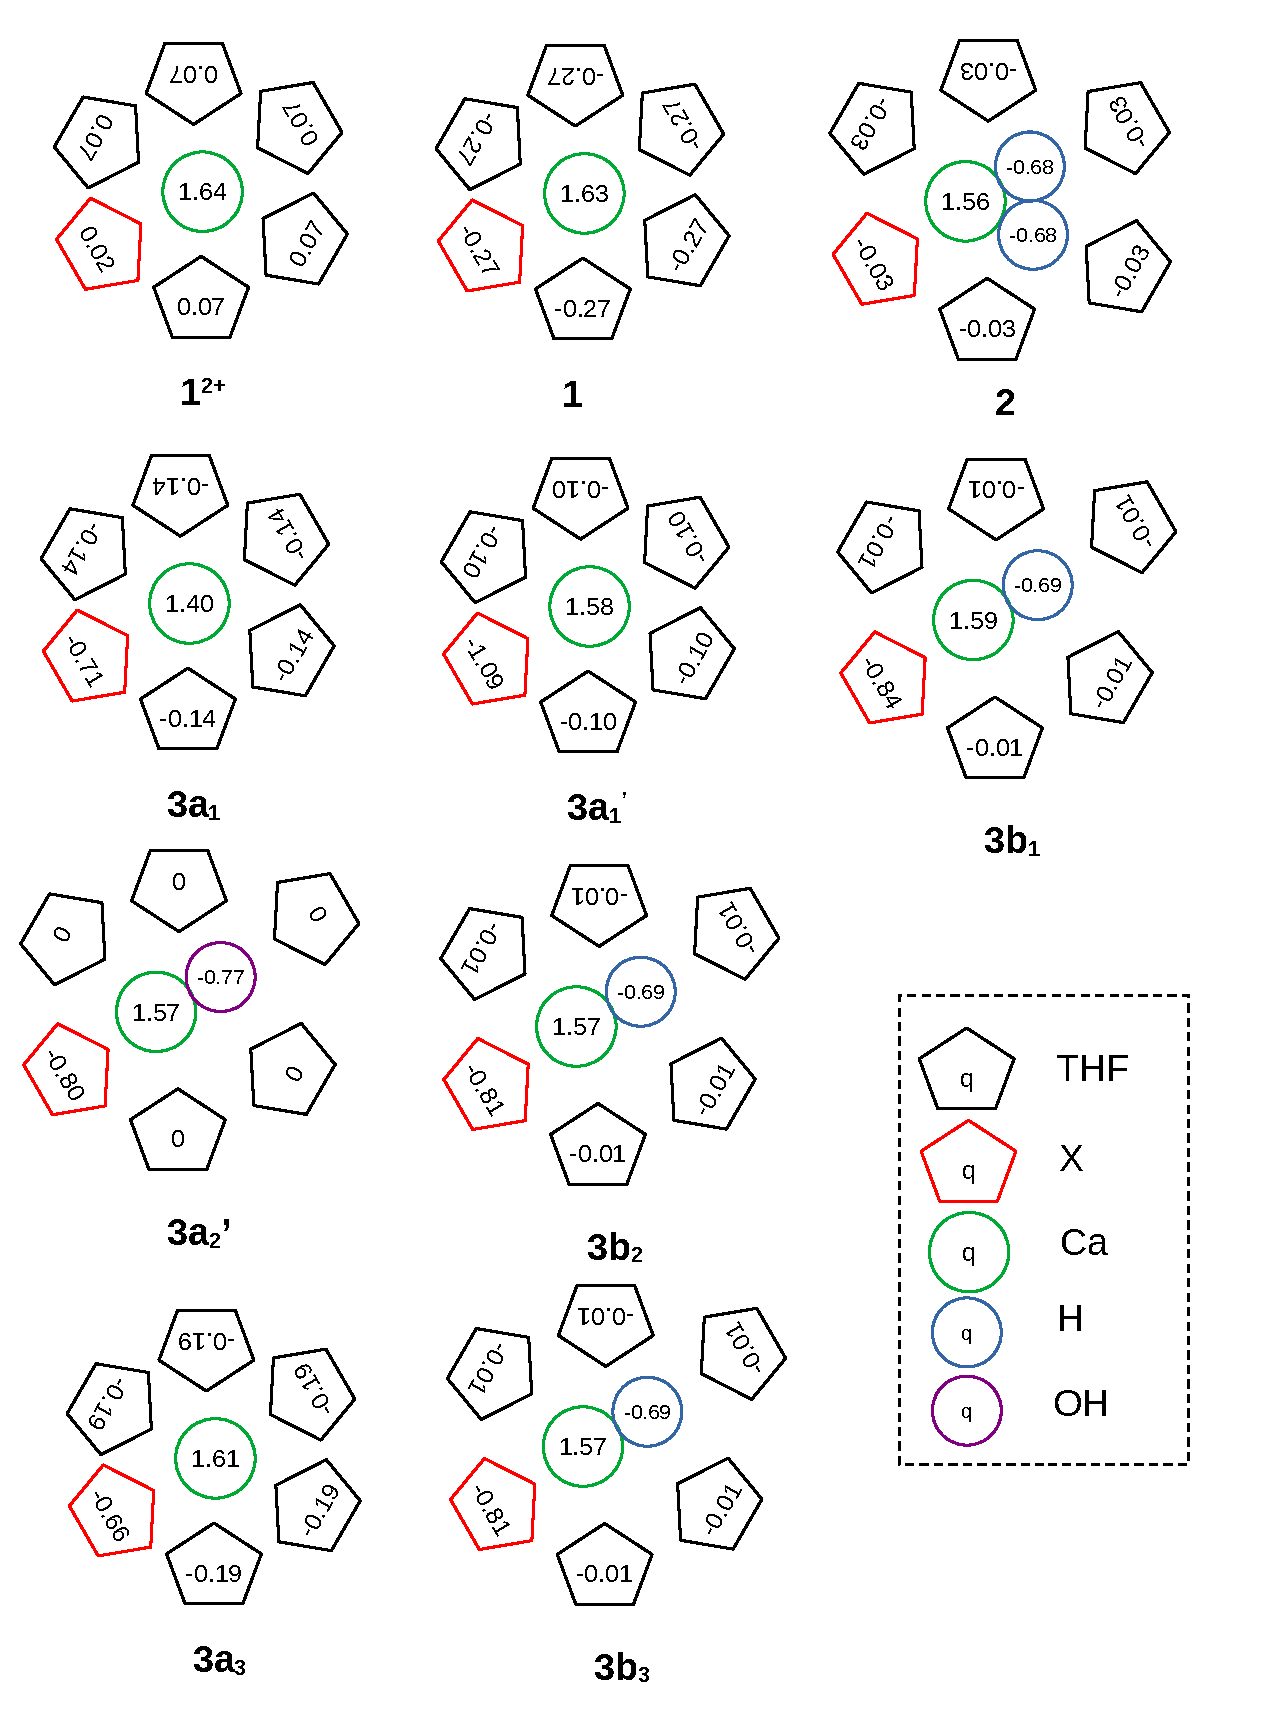
\includegraphics[width=\linewidth]{FigureS4}
\caption{QTAIM charge distribution of the different fragments (X denotes the degraded THF) for the various compounds, as computed using the \texttt{bader} program for the structures reported in Table~\ref{tab:dists} (and Table~1 of the main text).}
\end{figure}

\begin{figure}[!h]
\centering
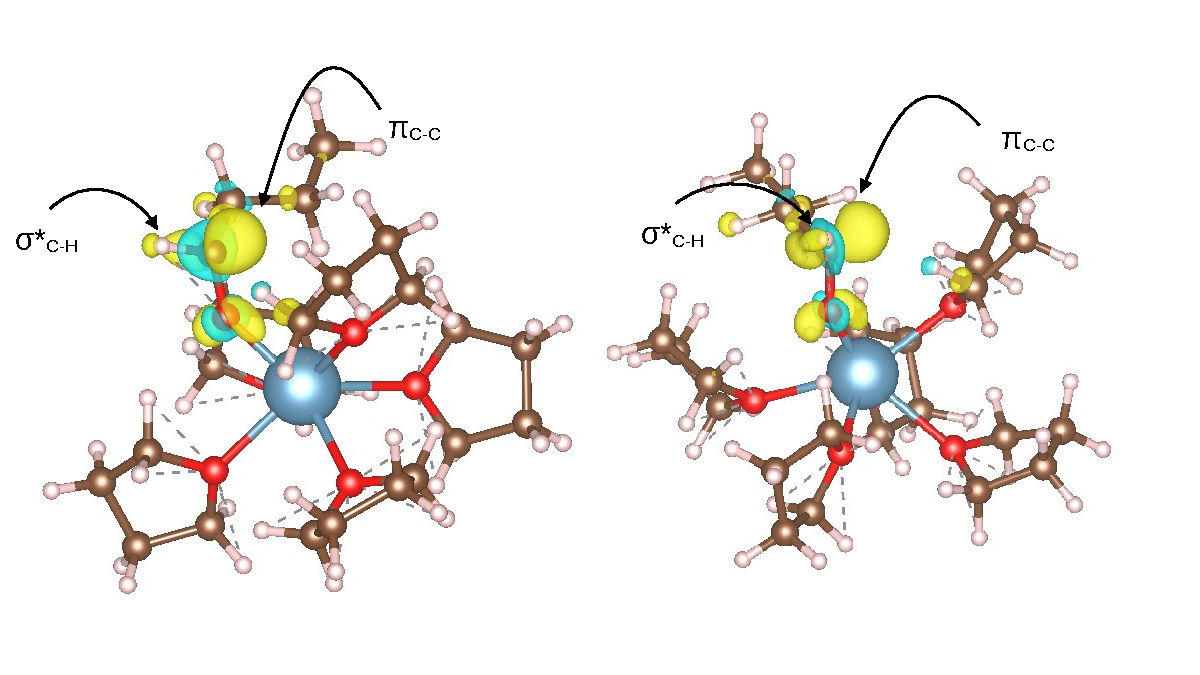
\includegraphics[width=\linewidth]{FigureS5}
\caption{Two different views (rotated by \SI{90}{\degree}) of the Fukui function ($f^{+}(\vec{r})$, $\Delta=\SI{0.4}{\elementarycharge}$, isocontour at \SI{8e-4}{\per\elementarycharge\cubed}) of \textbf{3a\textsubscript{1}'} at the reaction potential (\SI{-1.5}{\volt} vs SHE). Yellow (blue) regions indicate accumulation (depletion) of electron density, respectively.}
\end{figure}


\end{document}
